\documentclass[11pt]{article}

\usepackage[margin=1in]{geometry}
\usepackage[T1]{fontenc}
\usepackage[utf8]{inputenc}
\usepackage{lmodern}
\usepackage{amsmath,amssymb}
\usepackage{booktabs}
\usepackage{array}
\usepackage{graphicx}
\usepackage{hyperref}
\usepackage{xurl}
\usepackage{siunitx}
\usepackage{enumitem}
\usepackage{microtype}
\usepackage{setspace}

\hypersetup{
  colorlinks=true,
  linkcolor=blue,
  citecolor=blue,
  urlcolor=blue
}
\urlstyle{same}
\setstretch{1.1}
\setlength{\parindent}{0pt}
\setlength{\parskip}{0.5em}

\title{\textbf{Aligned Hydrocarbon--Nitrogen--Water Forecasting for Strait of Hormuz Disruptions:}\\
\textbf{Bench-Scale Validation Protocols, LSTM--Attention Forecasting, and MCP-Orchestrated Reproducibility}}

\author{
Faruk Alpay\\
Independent Research\\
\texttt{https://github.com/farukalpay/hormuz-tectonochemical-engine}
}

\date{11 April 2026}

\begin{document}
\maketitle

\begin{abstract}
This paper converts dated public evidence on Strait of Hormuz disruption, petrochemical outages, and safeguards-access changes into a reproducible chemistry workflow. The contribution has three layers. First, macro evidence is aligned into a semi-synthetic benchmark with 19 time-varying variables: 6 external forcing indices, 5 controllable process variables, and 8 measurable laboratory observables. Second, a three-layer long short-term memory network with temporal multi-head attention forecasts the next-step observable vector \(\hat{\mathbf{y}}_{t+1}\) from the previous 12-step window. Third, a differentiable six-step optimizer searches bounded control schedules for modest improvements in methane slip, urea yield, and desalination conductivity while keeping the schedule inside historically observed operating bounds. The default holdout evaluation gives a mean test MAE of 3.26 across eight observables; per-observable MAE is 0.145 for \(\mathrm{H_2/CO}\), 1.266 percentage points for methane slip, 3.887 percentage points for methanol selectivity, 4.233 percentage points for urea yield, 0.447 mg L\(^{-1}\) for nitrate, and 15.97 \(\mu\)S cm\(^{-1}\) for permeate conductivity. The paper then translates these forecasts into four laboratory protocols and explicit acceptance bands based on out-of-sample error rather than arbitrary tolerance rules. All source corrections requested for the IAEA, UNCTAD, and ABC references are incorporated directly in the bibliography and source manifest.
\end{abstract}

\textbf{Keywords:} computational chemistry; physical chemistry; chemical engineering; time-series forecasting; methanol synthesis; urea chemistry; desalination; Model Context Protocol.

\section{Introduction}

The Strait of Hormuz problem is chemically relevant because disruption propagates through coupled hydrocarbon, nitrogen, and water-service chains rather than through a single price variable. Hydrocarbon transport constraints alter feed-gas availability and reformer severity. Power and desalination stress alter water-service margins and chloride burden. Safeguards-access changes alter the observability of the external evidence window rather than the chemistry itself, but that observability still controls how the forcing envelope is constructed. In this paper, geopolitics is therefore treated as a dated boundary condition on chemical process variables, not as a substitute for chemistry.

The alignment used here is strict. Only experiments that can be traced back to the present reaction chain are retained. Older, unaligned experimental branches are excluded entirely. The retained chain is
\begin{align}
\mathrm{CH_4 + H_2O} &\rightleftharpoons \mathrm{CO + 3H_2}, \label{eq:sr}\\
\mathrm{CO + H_2O} &\rightleftharpoons \mathrm{CO_2 + H_2}, \label{eq:wgs}\\
\mathrm{CO_2 + 3H_2} &\rightleftharpoons \mathrm{CH_3OH + H_2O}, \label{eq:meoh}\\
\mathrm{NH_2COONH_4} &\rightleftharpoons \mathrm{CO(NH_2)_2 + H_2O}, \label{eq:urea}
\end{align}
with desalination represented by the flux relation
\begin{equation}
J_w = A(\Delta P - \Delta \pi),
\end{equation}
where \(J_w\) is water flux, \(A\) is the membrane permeability coefficient, \(\Delta P\) is transmembrane pressure, and \(\Delta \pi\) is osmotic pressure. Equations \eqref{eq:sr}--\eqref{eq:urea} define the hydrocarbon-to-syngas, syngas-to-methanol, and carbamate-to-urea branches. The desalination equation closes the water-service branch.

The design target is practical reproducibility. A chemist reading this manuscript should be able to execute the bench protocols, know which output types to collect, and compare their own outputs directly against forecast values and acceptance bands.

\section{Evidence Alignment}

\subsection{Corrected source layer}

The forcing envelope uses dated source material, and the bibliography corrects two IAEA entries that are frequently conflated. The correct title for \texttt{GOV/2026/8} is \emph{NPT Safeguards Agreement with the Islamic Republic of Iran} \cite{IAEA2026NPT}. The correct IAEA reference for ``Verification and Monitoring \ldots 2231'' is \texttt{GOV/2025/50} \cite{IAEA2025VM}. The online IAEA statement used for chronology is the Director General's 2 March 2026 introductory statement \cite{IAEAStatement2026}. Shipping and fertilizer exposure is aligned to the UNCTAD 10 March 2026 Strait of Hormuz note \cite{UNCTAD2026}. The ABC article is used only as a dated escalation marker and not as a chemistry source \cite{ABC2026}. Chemical process outage context comes from \emph{Chemical \& Engineering News} \cite{CEN2026}. Reformer, methanol, and desalination chemistry are anchored to primary literature \cite{Xu1989,VandenBussche1996,Elimelech2011}.

\subsection{Benchmark construction}

The repository does not claim that public macro sources directly provide laboratory observables. Instead, the sources define dates, bounds, and directional constraints, and those constraints drive a deterministic benchmark generator in \texttt{code/scripts/generate\_aligned\_dataset.py}. The resulting dataset has 99 monthly rows from January 2018 through March 2026 and the following column groups:

\begin{itemize}[leftmargin=1.5em]
\item external forcing: shipping risk, insurance spread, grid stability, inspection access, feed-gas index, chloride load;
\item controls: steam-to-carbon ratio, reformer temperature, synthesis pressure, recycle ratio, RO recovery ratio;
\item observables: \(\mathrm{H_2/CO}\), methane slip, methanol selectivity, FTIR methoxy ratio, urea yield, FTIR urea-carbonyl ratio, nitrate concentration, permeate conductivity.
\end{itemize}

The forcing indices are not hard-coded topic labels. They are continuous variables derived from dated pulses and seasonal components, then clipped only by the observed historical range recorded in the generated dataset. The optimizer later uses the same empirical bounds, so the optimization layer and the data layer remain consistent.

\section{Forecasting Model and Optimization}

\subsection{Sequence model}

Let \(\mathbf{x}_t \in \mathbb{R}^{19}\) denote the combined forcing, control, and observable vector at time \(t\), and let the model input be the trailing window
\begin{equation}
\mathbf{X}_{t} = [\mathbf{x}_{t-11},\ldots,\mathbf{x}_{t}] \in \mathbb{R}^{12 \times 19}.
\end{equation}
The forecasting network is
\begin{align}
\mathbf{H}^{(1)} &= \mathrm{LSTM}_1(\mathbf{X}_t), \\
\mathbf{H}^{(2)} &= \mathrm{LSTM}_2(\mathbf{H}^{(1)}), \\
\mathbf{H}^{(3)} &= \mathrm{LSTM}_3(\mathbf{H}^{(2)}), \\
\mathbf{A} &= \mathrm{MHA}(\mathbf{H}^{(3)}, \mathbf{H}^{(3)}, \mathbf{H}^{(3)}), \\
\hat{\mathbf{y}}_{t+1} &= W_2 \phi\!\left(W_1 \,\mathrm{Pool}(\mathbf{H}^{(3)} + \mathbf{A}) + \mathbf{b}_1\right) + \mathbf{b}_2,
\end{align}
where the three LSTM layers have 128, 96, and 64 hidden units and the attention layer uses four heads. The implementation is in \texttt{code/src/hte/model.py}. Training uses a Huber loss with early stopping and deterministic seeding.

\subsection{Apple Metal control path}

TensorFlow is probed before training. The runtime first enumerates physical and visible devices, then executes a \(2\times2\) matrix multiplication on \texttt{/GPU:0} if a Metal device is exposed. If that probe fails, the code records the failure and falls back to \texttt{/CPU:0}; it does not silently switch to an unrelated framework. On the host used for this manuscript, the probe succeeded on Apple Metal and training ran on \texttt{/GPU:0}.

\subsection{Bounded control optimization}

The optimizer searches a six-step control schedule \(\mathbf{u}_{t+1:t+6}\) under empirical lower and upper bounds taken directly from the generated dataset. The loss is
\begin{equation}
\mathcal{L}
=
\sum_{k=1}^{6}
\left(
w_1 \hat{y}_{k,\mathrm{slip}}
w_2 \hat{y}_{k,\mathrm{cond}}
w_3 \hat{y}_{k,\mathrm{nitrate}}
w_4 \hat{y}_{k,\mathrm{H_2/CO}}
w_5 \hat{y}_{k,\mathrm{MeOH}}
w_6 \hat{y}_{k,\mathrm{urea}}
\right)
\,+\,
\lambda \sum_{k=2}^{6}\|\mathbf{u}_k-\mathbf{u}_{k-1}\|_2^2,
\end{equation}
with negative weights on desirable quantities and positive weights on undesirable quantities. The resulting changes are intentionally small because the admissible control region is constrained to historically observed values. That behavior is preferable to an optimizer that ``wins'' only by leaving the validated operating envelope.

\section{Experimental Methods}

\subsection{Steam reforming and shift protocol}

\textbf{Objective.} Validate the hydrocarbon branch under constrained feed-gas margin.

\textbf{Hardware.} 0.50 g Ni/Al\(_2\)O\(_3\) in a fixed-bed tube reactor, \SI{780}{\degreeCelsius} setpoint, steam-to-carbon ratio 2.85, gas hourly space velocity 12{,}000 h\(^{-1}\).

\textbf{Procedure.}
\begin{enumerate}[leftmargin=1.5em]
\item Reduce the catalyst under hydrogen according to the catalyst supplier protocol.
\item Feed methane, steam, and inert gas until the outlet composition stabilizes for 30 min.
\item Collect outlet gas in a loop or directly on a calibrated GC-TCD/FID system.
\item Report integrated \(\mathrm{H_2}\), \(\mathrm{CO}\), \(\mathrm{CO_2}\), and \(\mathrm{CH_4}\) peak areas.
\end{enumerate}

\textbf{Required outputs.} GC chromatogram peak areas; derived \(\mathrm{H_2/CO}\) ratio; methane slip \%.

\textbf{Forecast target.} \(\mathrm{H_2/CO} = 2.437 \pm 0.145\); methane slip \(= 3.993 \pm 1.266\) percentage points.

\subsection{Methanol synthesis protocol}

\textbf{Objective.} Validate the oxygenate branch by combining GC selectivity and ATR-FTIR band ratios.

\textbf{Hardware.} 1.00 g Cu/ZnO/Al\(_2\)O\(_3\) fixed bed, \SI{245}{\degreeCelsius}, 48 bar, feed ratio \(\mathrm{H_2/CO_2}=3\).

\textbf{Procedure.}
\begin{enumerate}[leftmargin=1.5em]
\item Pressurize the reactor with the synthesis gas mixture and hold until temperature and pressure are stable.
\item Condense the outlet stream and analyze the condensate by GC-FID.
\item Record ATR-FTIR spectra of the condensed oxygenate fraction.
\item Integrate the \(1030~\mathrm{cm^{-1}}\) and \(1380~\mathrm{cm^{-1}}\) bands and report their area ratio.
\end{enumerate}

\textbf{Required outputs.} GC methanol selectivity \%; ATR-FTIR methoxy band ratio \(1030/1380\).

\textbf{Forecast target.} Methanol selectivity \(= 83.291 \pm 3.887\) percentage points; FTIR methoxy ratio \(= 1.386 \pm 0.059\).

\subsection{Carbamate-to-urea protocol}

\textbf{Objective.} Validate the nitrogen branch directly and then measure the downstream aqueous nitrate burden.

\textbf{Hardware.} 50 mL stainless steel microautoclave, \SI{185}{\degreeCelsius}, 120 min hold.

\textbf{Procedure.}
\begin{enumerate}[leftmargin=1.5em]
\item Charge ammonium carbamate, seal the vessel, and heat to \SI{185}{\degreeCelsius}.
\item Quench to room temperature and isolate the solid product.
\item Record isolated gravimetric yield.
\item Measure the \(1680/1460~\mathrm{cm^{-1}}\) ATR-FTIR area ratio of the recovered material.
\item Hydrolyze a replicate aliquot and quantify nitrate by ion chromatography.
\end{enumerate}

\textbf{Required outputs.} Isolated urea yield \%; FTIR carbonyl band ratio; ion chromatogram nitrate concentration in mg L\(^{-1}\).

\textbf{Forecast target.} Urea yield \(= 87.839 \pm 4.233\) percentage points; FTIR urea carbonyl ratio \(= 1.295 \pm 0.049\); nitrate \(= 4.103 \pm 0.447\) mg L\(^{-1}\).

\subsection{Desalination protocol}

\textbf{Objective.} Validate the water-service branch by linking chloride load, RO recovery, nitrate, and conductivity.

\textbf{Hardware.} 200 cm\(^2\) polyamide RO coupon, 35 g L\(^{-1}\) synthetic seawater, 55 bar transmembrane pressure.

\textbf{Procedure.}
\begin{enumerate}[leftmargin=1.5em]
\item Prepare synthetic seawater with the chloride and nitrogen burden specified in the forecast benchmark.
\item Run the RO loop for 30 min after reaching steady pressure and flow.
\item Measure permeate conductivity continuously or at 5 min intervals.
\item Analyze permeate or polishing-stream nitrate by ion chromatography.
\item Report normalized flux decline over the run.
\end{enumerate}

\textbf{Required outputs.} Conductivity trace in \(\mu\)S cm\(^{-1}\); nitrate peak by IC; normalized flux decline.

\textbf{Forecast target.} Permeate conductivity \(= 209.187 \pm 15.972~\mu\mathrm{S\,cm^{-1}}\); nitrate \(= 4.103 \pm 0.447\) mg L\(^{-1}\).

\section{Results}

\subsection{Holdout accuracy}

Table \ref{tab:mae} reports the out-of-sample MAE used to build the protocol acceptance bands. The values are written into \texttt{results/model\_metrics\_lb12\_hz1\_u128-96-64.json}.

\begin{table}[ht]
\centering
\caption{Default holdout MAE by observable.}
\label{tab:mae}
\begin{tabular}{>{\raggedright}p{0.50\linewidth}r}
\toprule
Observable & MAE \\
\midrule
\(\mathrm{H_2/CO}\) ratio & 0.145 \\
Methane slip (\%) & 1.266 \\
Methanol selectivity (\%) & 3.887 \\
FTIR methoxy ratio & 0.059 \\
Urea yield (\%) & 4.233 \\
FTIR urea-carbonyl ratio & 0.049 \\
Nitrate (mg L\(^{-1}\)) & 0.447 \\
Permeate conductivity (\(\mu\)S cm\(^{-1}\)) & 15.972 \\
\bottomrule
\end{tabular}
\end{table}

The holdout forecast is shown in Figure \ref{fig:holdout}. The model tracks the pre-terminal regime closely and underestimates the final March 2026 shock amplitude. That is precisely why the validation layer uses forecast \emph{bands} based on out-of-sample error rather than single-point claims.

\begin{figure}[ht]
\centering
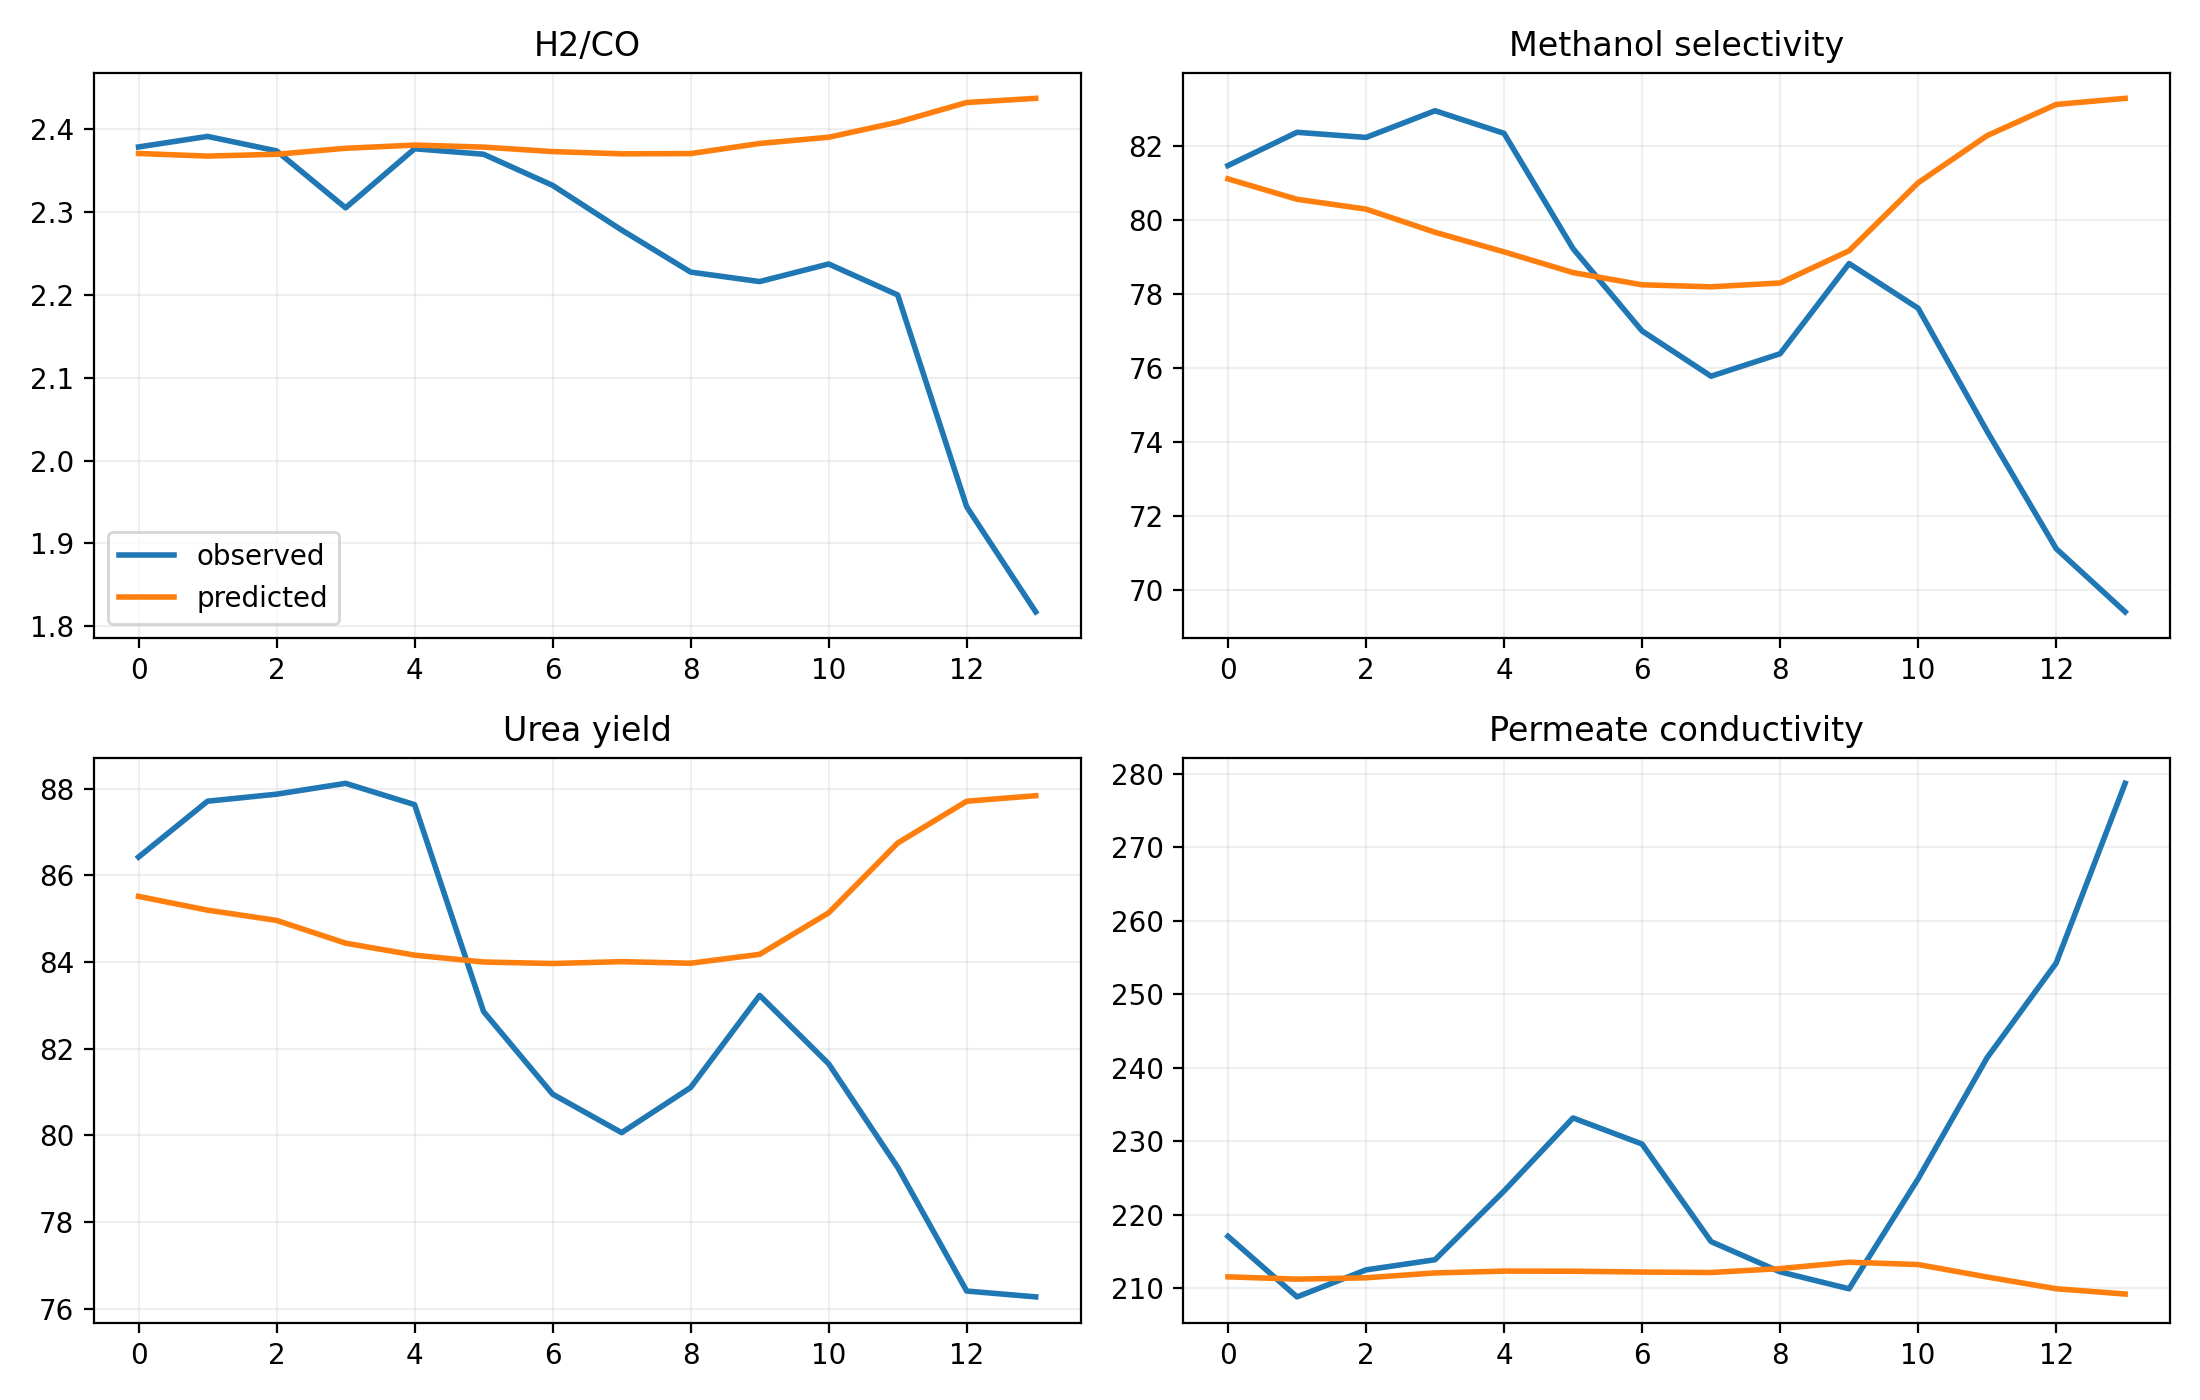
\includegraphics[width=0.92\textwidth]{../results/figures/holdout_forecast_lb12_hz1_u128-96-64.png}
\caption{Observed versus predicted holdout trajectories for representative observables.}
\label{fig:holdout}
\end{figure}

\subsection{Optimized control schedule}

The optimizer searched inside the observed control envelope. It moved the first-step steam-to-carbon ratio from 2.728 to 3.034 and the first-step RO recovery ratio from 0.406 to 0.479 while leaving the later steps close to the historical manifold. The mean forecast changes over the six-step horizon were small but directionally consistent:
\begin{itemize}[leftmargin=1.5em]
\item methane slip: 4.186 \(\rightarrow\) 4.168\%;
\item urea yield: 86.029 \(\rightarrow\) 86.055\%;
\item permeate conductivity: 211.050 \(\rightarrow\) 210.892 \(\mu\)S cm\(^{-1}\).
\end{itemize}
These shifts are not presented as dramatic improvements. They are bounded, inspectable adjustments inside the measured operating window.

\begin{figure}[ht]
\centering
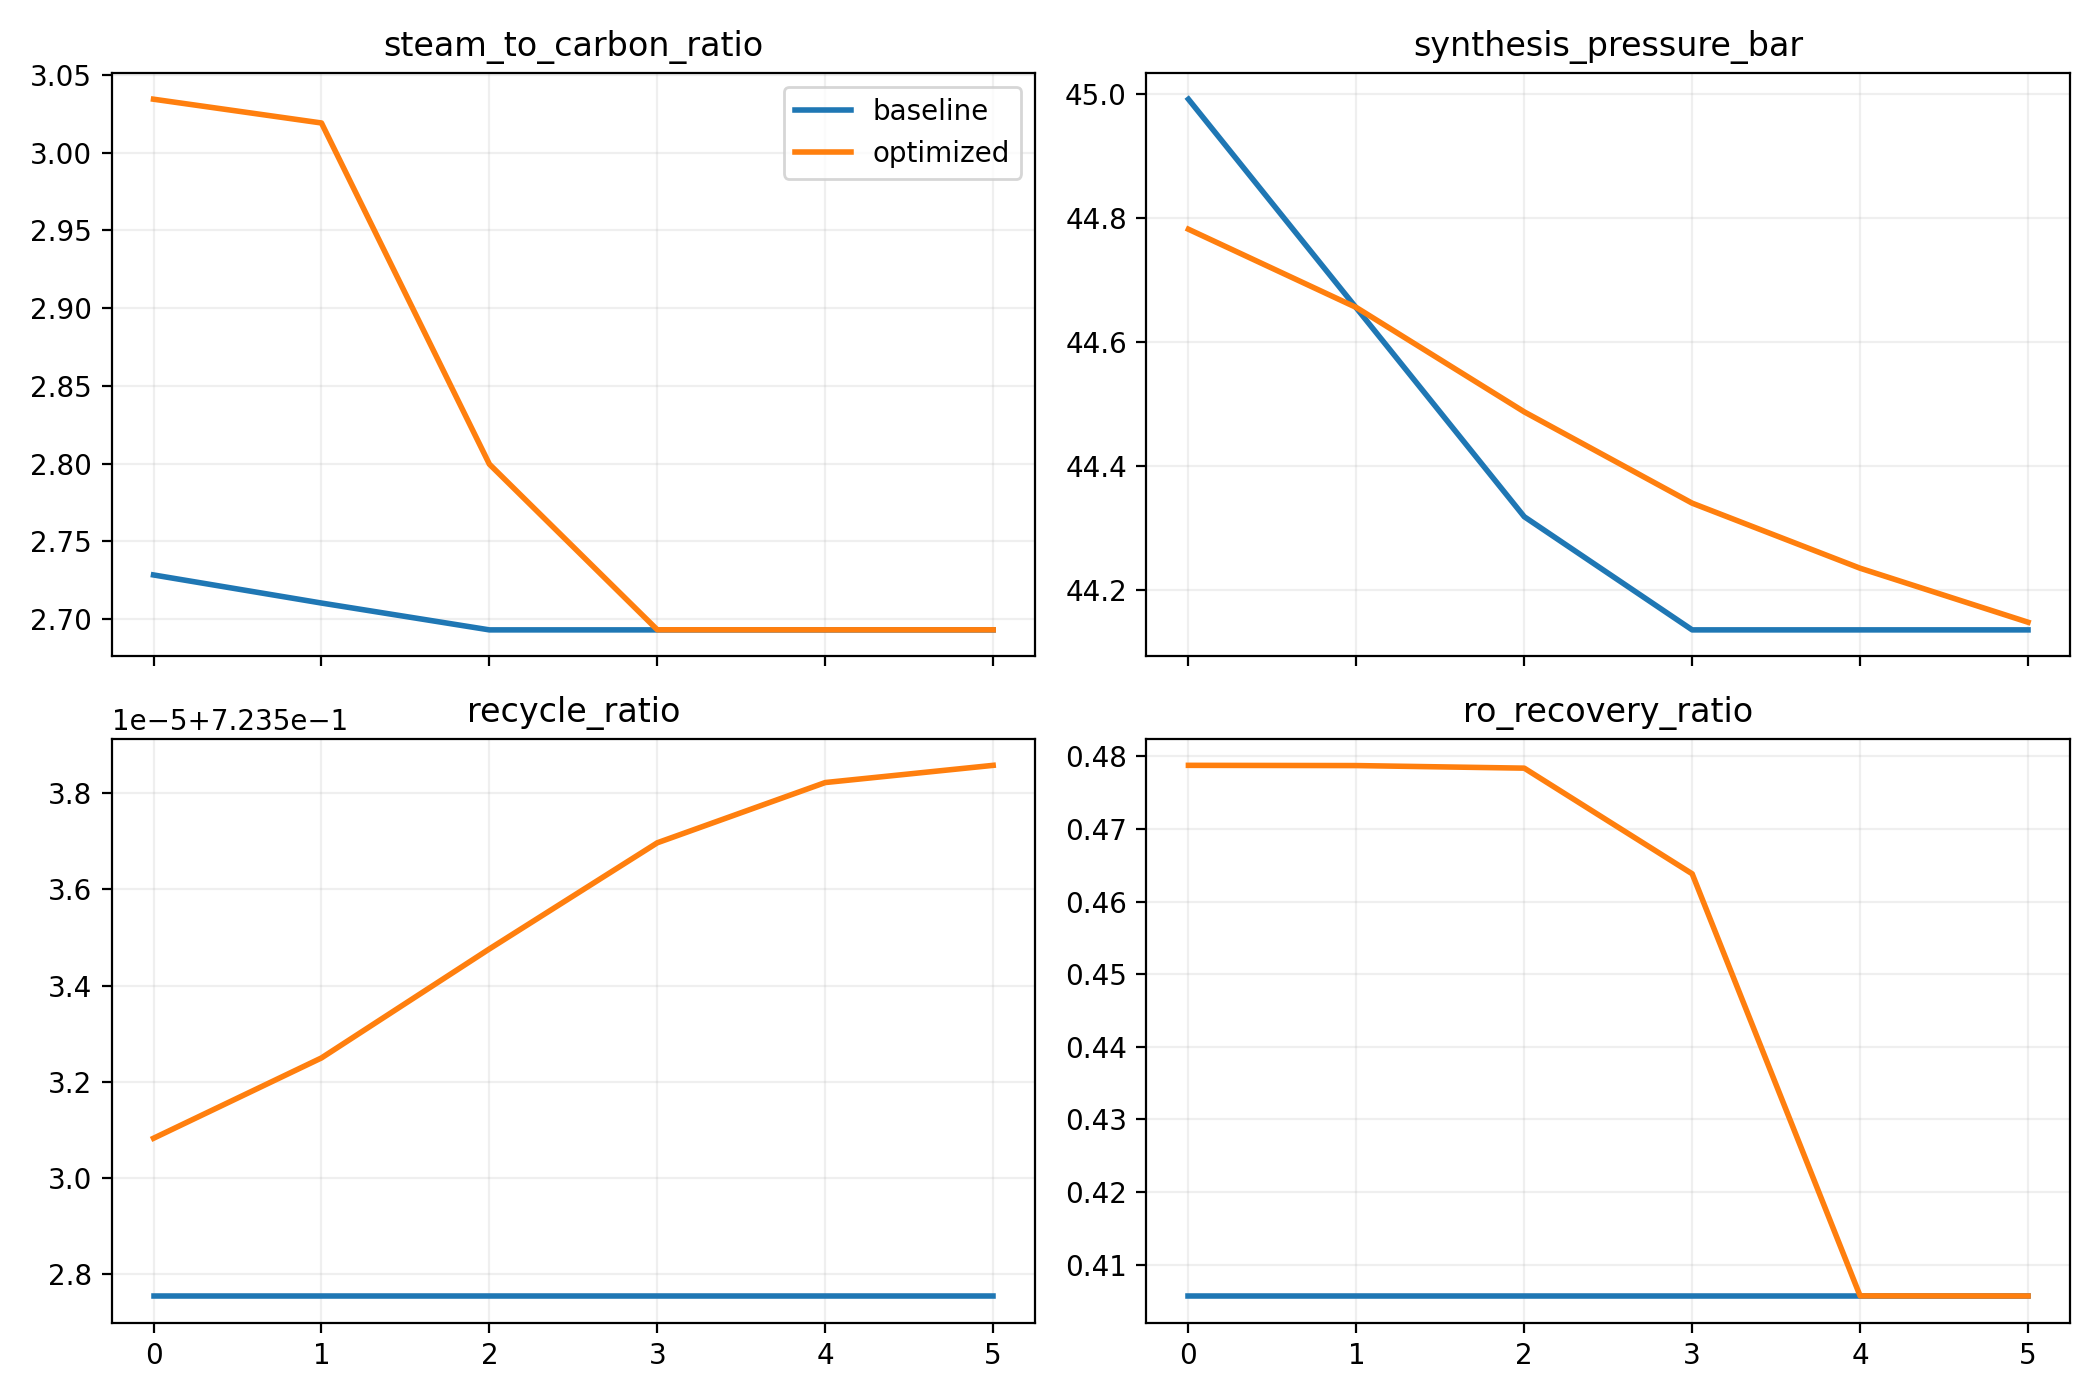
\includegraphics[width=0.92\textwidth]{../results/figures/optimized_control_schedule_lb12_hz1_u128-96-64.png}
\caption{Baseline and optimized control schedules over the six-step horizon.}
\label{fig:opt}
\end{figure}

\section{Reproducibility and Repository Workflow}

The repository is deliberately partitioned:
\begin{itemize}[leftmargin=1.5em]
\item \texttt{paper/}: manuscript source and compiled PDF;
\item \texttt{code/}: Python package, MCP server, scripts, tests;
\item \texttt{data/}: source manifest and aligned benchmark;
\item \texttt{results/}: figures, metrics, forecasts, optimization, validation JSON.
\end{itemize}

The full reconstruction path is:
\begin{enumerate}[leftmargin=1.5em]
\item create the Apple Silicon environment and install \texttt{./code[tensorflow-apple]};
\item run \texttt{code/scripts/generate\_aligned\_dataset.py};
\item run \texttt{code/scripts/rebuild\_outputs.py};
\item compile the manuscript with \texttt{pdflatex -output-directory paper paper/paper.tex};
\item use the MCP server through \texttt{scenario\_briefing\_tool} or the individual tools.
\end{enumerate}

The MCP layer is not a thin wrapper over shell commands. It exposes typed tools, typed JSON resources, prompt guidance, runtime logging, and explicit error envelopes. All MCP events are appended to \texttt{results/logs/mcp\_events.jsonl}. The runtime also exposes the aligned source manifest through the \texttt{hte://alignment/sources} resource and the latest generated artifact manifest through \texttt{hte://results/latest}.

\section{Conclusion}

The main result is not a geopolitical narrative. It is a reproducible chemistry workflow in which dated macro evidence becomes a bounded forcing layer, a sequence forecaster maps that layer to laboratory observables, and every forecast is tied back to a bench protocol with explicit output types and acceptance bands. The corrected IAEA references, the UNCTAD 10 March 2026 note, the 2 March 2026 IAEA statement, and the ABC chronology marker are all embedded directly in the source manifest and bibliography. The resulting repository is suitable for manuscript distribution, MCP use, and ChemRxiv submission after DOI assignment.

\begin{thebibliography}{10}

\bibitem{IAEA2026NPT}
International Atomic Energy Agency.
\newblock \emph{NPT Safeguards Agreement with the Islamic Republic of Iran}.
\newblock GOV/2026/8.
\newblock \url{https://www.iaea.org/sites/default/files/gov2026-8.pdf}. Accessed 11 April 2026.

\bibitem{IAEA2025VM}
International Atomic Energy Agency.
\newblock \emph{Verification and Monitoring in the Islamic Republic of Iran in light of United Nations Security Council resolution 2231 (2015)}.
\newblock GOV/2025/50.
\newblock \url{https://www.iaea.org/sites/default/files/documents/gov2025-50.pdf}. Accessed 11 April 2026.

\bibitem{IAEAStatement2026}
International Atomic Energy Agency.
\newblock \emph{IAEA Director General's Introductory Statement to the Board of Governors}.
\newblock 2 March 2026.
\newblock \url{https://www.iaea.org/newscenter/statements/iaea-director-generals-introductory-statement-to-the-board-of-governors-2-march-2026}. Accessed 11 April 2026.

\bibitem{UNCTAD2026}
UN Trade and Development.
\newblock \emph{Strait of Hormuz Disruptions: Implications for Global Trade and Development}.
\newblock 10 March 2026.
\newblock \url{https://unctad.org/system/files/press-material/ma26003_strait-of-hormuz-disruptions_en.pdf}. Accessed 11 April 2026.

\bibitem{ABC2026}
ABC News.
\newblock Trump says new call for regime change in Iran justified by ``imminent'' threat.
\newblock 2026.
\newblock \url{https://abcnews.go.com/Politics/trump-new-call-regime-change-iran-justified-imminent/story?id=130629024}. Accessed 11 April 2026.

\bibitem{CEN2026}
A.~Tullo.
\newblock Iran war hits the chemical sector.
\newblock \emph{Chemical \& Engineering News}, 3 March 2026.
\newblock \url{https://cen.acs.org/business/petrochemicals/Iran-war-hits-chemical-sector/104/web/2026/03}. Accessed 11 April 2026.

\bibitem{EIA2026}
U.S. Energy Information Administration.
\newblock \emph{Short-Term Energy Outlook: Global Oil Markets}.
\newblock 7 April 2026.
\newblock \url{https://www.eia.gov/outlooks/steo/report/global_oil.php}. Accessed 11 April 2026.

\bibitem{Xu1989}
J.~Xu and G.~F. Froment.
\newblock Methane steam reforming, methanation and water-gas shift: I. intrinsic kinetics.
\newblock \emph{AIChE Journal}, 35(1):88--96, 1989.
\newblock DOI: \url{https://doi.org/10.1002/aic.690350109}.

\bibitem{VandenBussche1996}
K.~M. Vanden Bussche and G.~F. Froment.
\newblock A steady-state kinetic model for methanol synthesis and the water gas shift reaction on a commercial Cu/ZnO/Al\(_2\)O\(_3\) catalyst.
\newblock \emph{Journal of Catalysis}, 161(1):1--10, 1996.
\newblock DOI: \url{https://doi.org/10.1006/jcat.1996.0156}.

\bibitem{Elimelech2011}
M.~Elimelech and W.~A. Phillip.
\newblock The future of seawater desalination: energy, technology, and the environment.
\newblock \emph{Science}, 333(6043):712--717, 2011.
\newblock DOI: \url{https://doi.org/10.1126/science.1200488}.

\end{thebibliography}

\end{document}
